\openingarticle
\def\ppages{\pagerange{WESIPS:firstpage}{WESIPS:lastpage}}
\def\shorttitle{Conference Review: Warfare, Environment, Social Inequality and Peace Studies}
\def\maintitle{Warfare, Environment, Social Inequality and Peace Studies Seville, Spain: May 29--30, 2015}
\def\shortauthor{Mariana Favila Vázquez, Ximena Chávez Balderas}
\def\authormail{}
\def\affiliation{}
\def\thanknote{}
%--------------------------------------------------------------
\mychapter{\maintitle}
\begin{center}
	{\Large\scshape Mariana Favila Vázquez\footnote{Mariana Favila Vázquez is an archaeologist by the National School of Anthropology and History in Mexico. She has a Master in Mesoamerican Studies by the National Autonomous University of Mexico (UNAM). Her research topic is the pre-Hispanic Mesoamerican navigation. She has participated in archaeological projects in the basin of Mexico and in the Maya area. She is currently a lecturer in the National School of Anthropology and History and is studying her doctorate in Mesoamerican Studies at UNAM.}} \\ \href{mailto:mariana.favila@gmail.com}{mariana.favila@gmail.com}\\
		National School of Anthropology and History, Mexico\\[1em]
	{\Large\scshape 	Ximena Chávez Balderas\footnote{Ximena Chávez Balderas is a bioarchaeologist at the Templo Mayor Project. She is specialized in funerary archaeology, sacrificial practices, mortuary treatments and archaeozoology. She earned her BA from the Escuela Nacional de Antropología e Historia. Her MPhil was awarded by the Universidad Nacional Autónoma de México and her MA by Tulane University. She is PhD candidate at Tulane University. She was the main curator of the Templo Mayor Museum between 2001 and 2007. She received three INAH national awards for her BA thesis, her MPhil thesis and for an exhibition she curated in 2006. She has presented more than eighty lectures and conference papers and has published some forty articles as well as a volume on funerary rituals—specifically cremation—at the Templo Mayor. Currently, she is working in two books, one as author and the other as editor. Chávez Balderas has worked on a number of national and international exhibitions and has excavated at Teotihuacan (including Teopancazco, Xalla, and the Pyramids of the Moon and the Sun), Loma Guadalupe in Michoacán, Huacas de Moche, Peru, and the Great Temple of Tenochtitlan.}}\\ \href{mailto:xchavezb@tulane.edu}{xchavezb@tulane.edu}\\
		Tulane University
\end{center}
\vspace{3em}
\midarticle
%--------------------------------------------------------------
\label{WESIPS:firstpage}
%---------------------------------------------------------------------------------------
	
	
\lettrine[nindent=0em,lines=3]{T}{he} Warfare, Environment, Social Inequality and Peace Studies (WESIPS) Conference was celebrated at the Center for Cross-Cultural Study (Spanish Studies Abroad) in Seville, Spain. Thanks to the great effort of organizers Dr. Richard J. Chacon (Winthrop University) and Dr. Yamilette Chacon (James Madison University), around 70 researchers from diverse countries, such as France, Germany, Mexico, Israel, the USA, England, Belgium, Peru, Australia, Sweden and Spain, met in this amazing city, defined as a cosmopolitan center during the sixteenth and seventeenth centuries. Anthropologists, biologists, archaeologists, psychologists, historians, graduate students, and independent scholars presented their concerns, as well as different theoretical and methodological perspectives on the origin, development and consequences that violence, social inequality, and warfare have on the environment and societies throughout history. In this review we will discuss selected topics presented in this conference and some of the papers that we believe reflect the main goals of this academic meeting. 

%\section{The study of ancient violence patterns}

Research\marginnote{The study of ancient violence patterns} on these topics was considered from economic, environmental, historical and social approaches. Archaeological research allows us to examine patterns of conflict and violence through the analysis of individual and collective actors, sociopolitical conditions and group affiliations as reflected in the material culture. However, evidence from other sources needs to be incorporated in order to interpret this data, making interdisciplinary approaches necessary. This approach was reflected in the conference proceedings. Peter Eeckhout (Université Libre de Bruxelles) and Lawrence Owens (University of London) presented “\textit{From domestic to ritual and beyond: evidence for conflict and violence at Pachacamac, Peru}”. The authors created an interpretative framework based on the analysis of archaeological remains, iconography, bioarchaeology and ethnohistorical data, allowing them to identify the manifestations of violence at different scales (interpersonal, socio-cultural, and state-sponsored). This concern, shared with other researchers, seeks to investigate the causes and patterns of warfare, as indicated by Elizabeth Arkush (University of Pittsburgh) in her paper "\textit{Patterns of warfare in the Pre-Columbian Andes at the large scale and the long term: horizons, variation, and causality}". She proposed the development of a GIS database to create a model for large-scale analysis which would create a visual of various indications of warfare, such as congregations of fortifications, settlement patterns and skeletal trauma rates for the Pre-Columbian Central Andes. On the other hand, research by Ximena Chávez Balderas (Instituto Nacional de Antropología e Historia), Alan Barrera (Instituto Nacional de Antropología e Historia) and Diana Bustos (Universidad Nacional Autónoma de México) “\textit{Sacrificial victims at Aztec Tenochtitlan: Captive warriors or slaves?}” reached an interesting conclusion. Their research suggested that violence is not necessarily connected to warfare and conflict, but rather could be related to standardized patterns of ritual violence, in order to reenact mythical events (Fig. \ref{fig:WESIPS_Fig1}).

	\begin{figure}[!htb]
		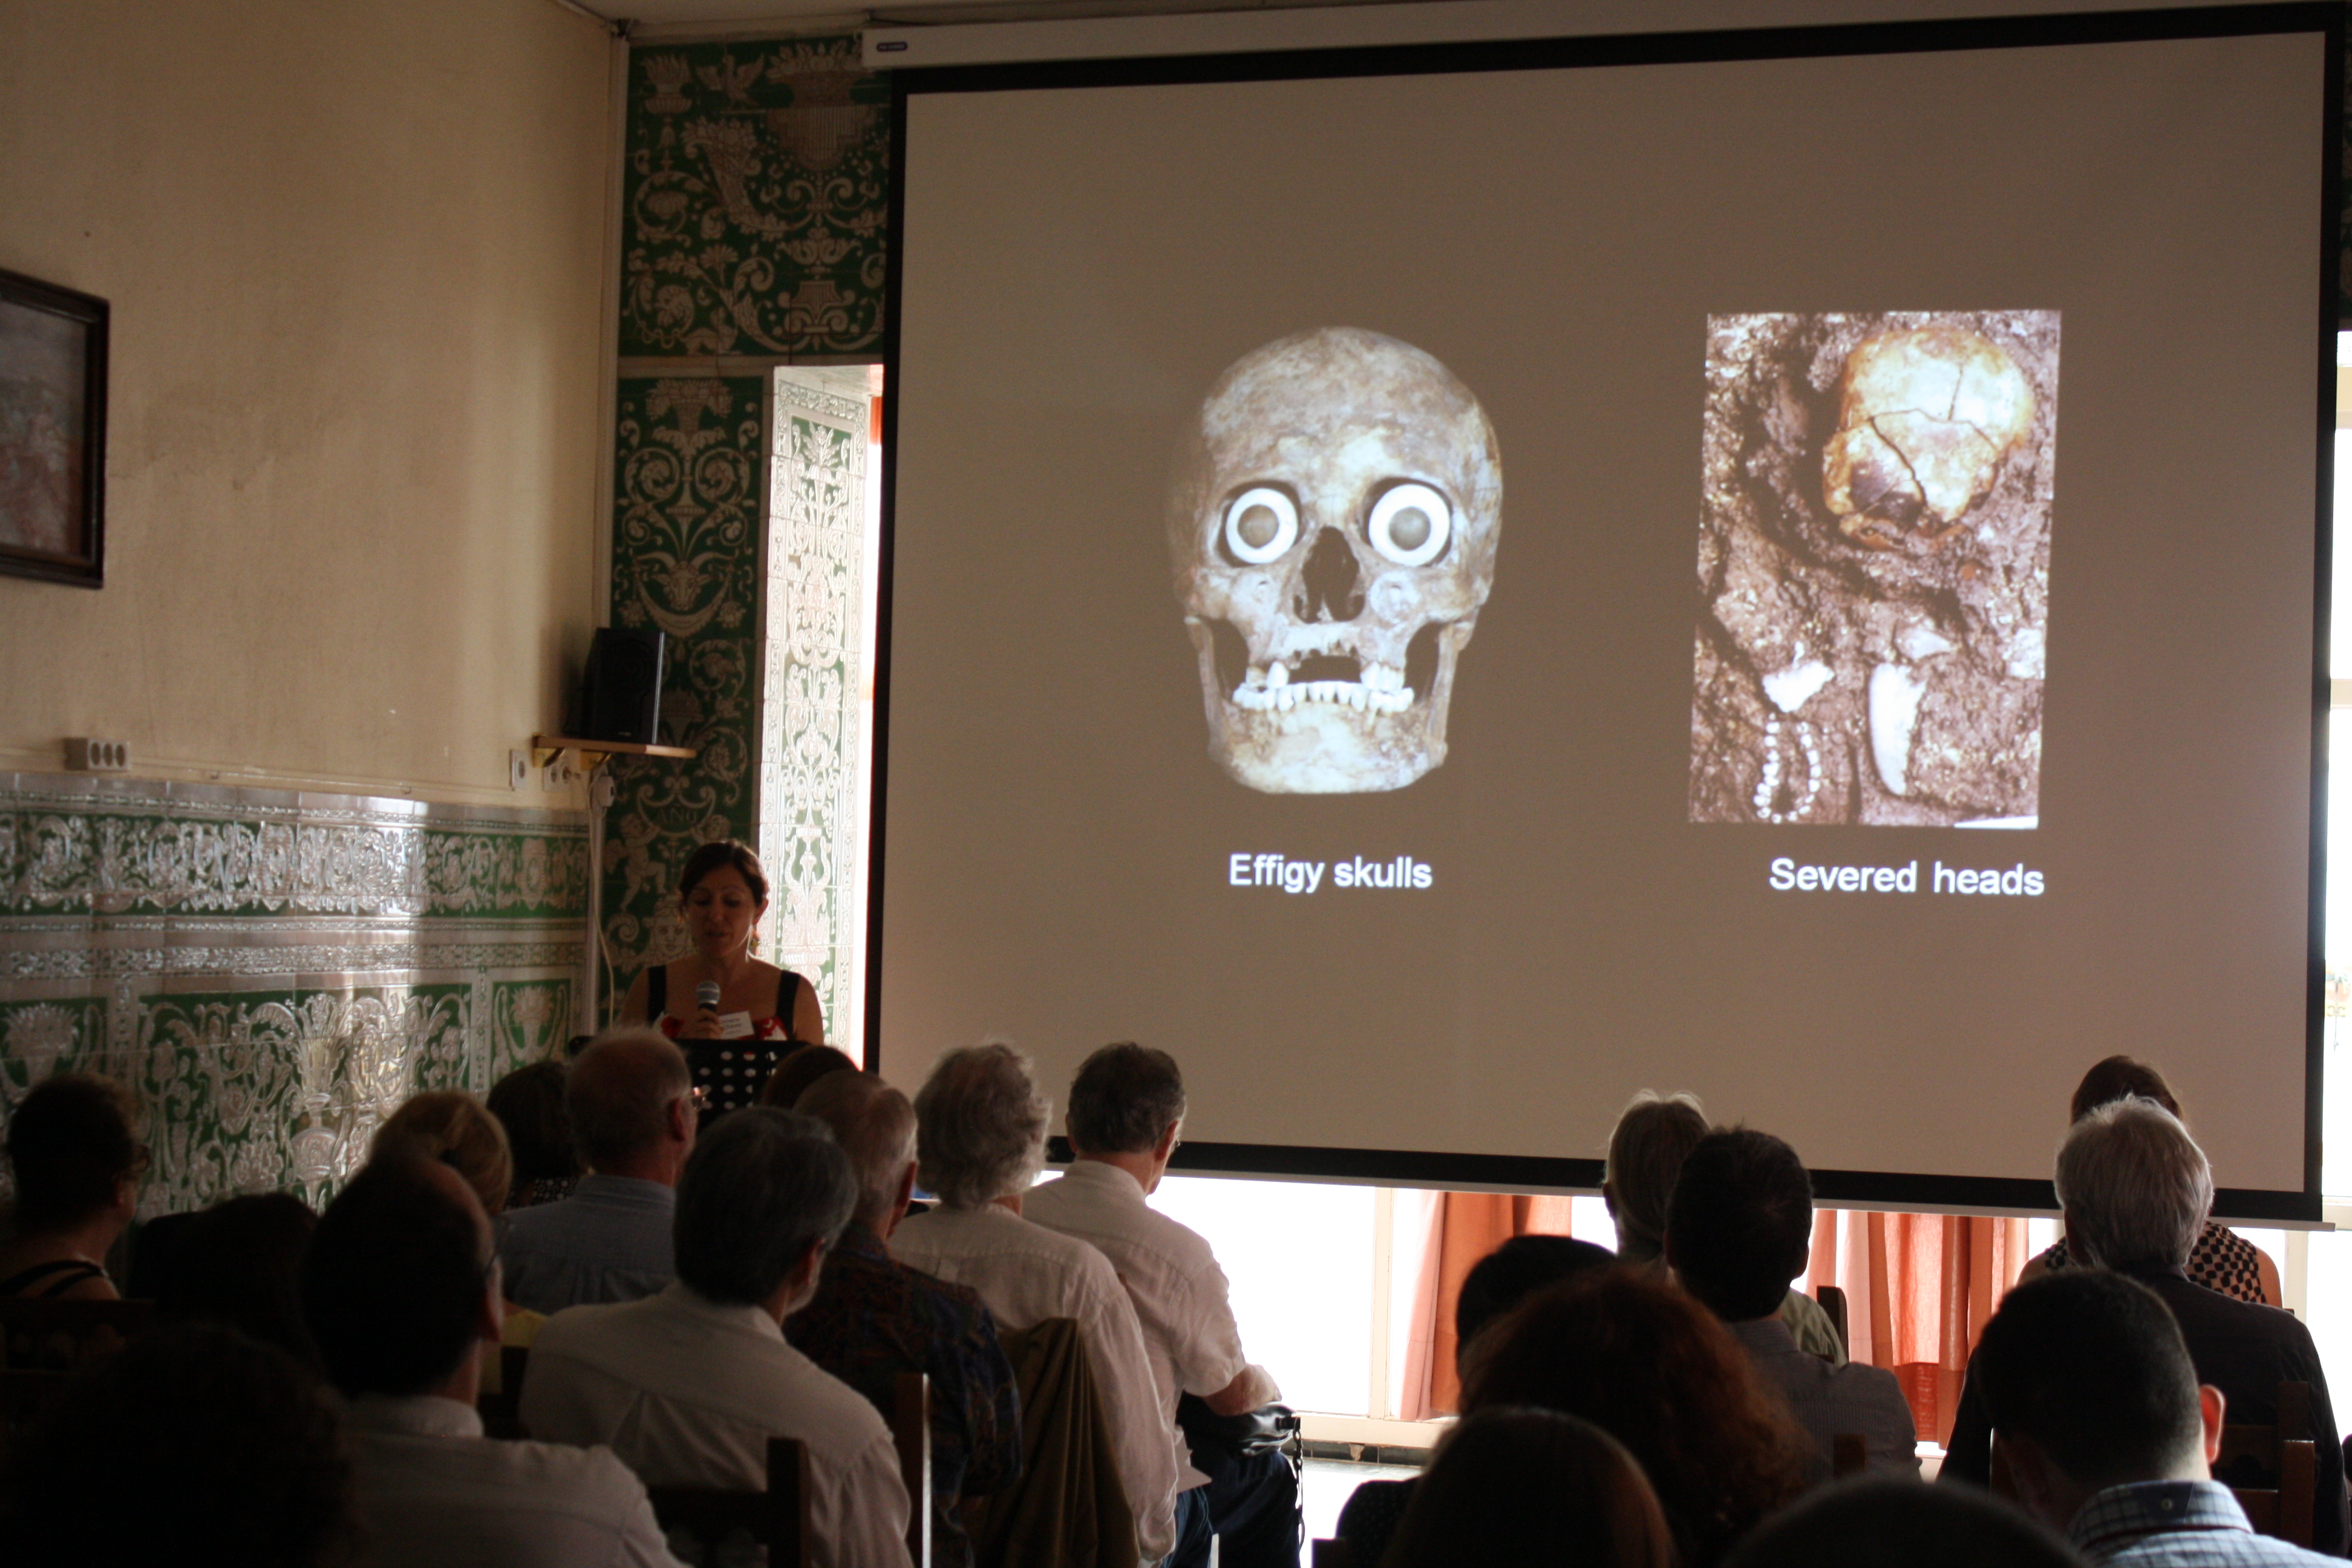
\includegraphics[width=.95\linewidth]{figures/WESIPS_Fig1.jpg}
		\centering
		\caption{Ximena Chávez presenting her paper about sacrificial victims in Tenochtitlan. Courtesy of Dr. Richard Chacon.}
		\label{fig:WESIPS_Fig1}
	\end{figure}

%\section{Conflict, conservation and environmental management}

When\marginnote{Conflict, conservation and environmental management} we think about conflict, environmental conservation is not taken into account on a regular basis. By exploring the relationship between these concepts from an anthropological and a historical point of view we will be able to understand environmental management. As stated by Charles Bishop (Union College) in his paper “\textit{Conservation and Territoriality among Northern Algonquians}”, what we call conservation today depends on territorial concepts; unfortunately this does not mean that all forms of territoriality resulted in conservation. How can we address the complex topic of territory and resource management?  Rubén Mendoza (California State University, Monterey Bay) and Jennifer Lucido (Sonoma State University) in their paper “\textit{Cartographies of Sustainability: A Geospatial and Digital Resource based Approach to the Visualization of the Environmental History of California, 1769- 1892}”, established a project based in environmental history and historical geography. Through the analysis of maps the authors obtained environmental histories of resource abundance and scarcity, connected to the water crisis. 

%\section{Maritime strategies: warfare and trade}

Maritime\marginnote{Maritime strategies: warfare and trade} routes have been documented around the world through rock art, codices, written documents, ship wrecks and other archaeological findings. This activity was pursued for two main objectives, warfare and trade, both intrinsically connected. This connection was confirmed in the paper “\textit{Rock Art, Warfare and Long Distance Trade}” by Johan Ling (University of Göthenburg) and Kristian Kristiansen (University of Gothenburg). The authors demonstrated that Scandinavian local warriors would have increasingly played an important role in the metal trade. In consequence, this privileged the rise of maritime chiefdoms in Scandinavia. In the paper “\textit{Nautical Warfare in Mesoamerica: Conquering through Water}”, Mariana Favila Vázquez (Universidad Nacional Autónoma de México) pointed out that the understanding of the nature and variability of Mesoamerican battles is still limited. However, there is enough evidence to conclude that nautical warfare synergistically occurred along with terrestrial warfare. As a result lacustrine and maritime landscapes became part of the political territories during Pre-Hispanic times. 

%\section{The study of conflict through the analysis of defensive architecture}

Conflict\marginnote{The study of conflict through the analysis of defensive architecture} can be identified through the study of different construction systems. For example, researchers are well aware that the period preceding the Inca Empire was characterized by conflict and warfare. This can be attested by the existence of numerous fortifications. However, the northern coast and the highlands were “far from adopting the same defensive patterns”. In the paper “\textit{Pucara VS Fortress: Defensive Arrangements during the Late Intermediate Period in the Coast and the Sierra of Central Andes},” Vincent Chamussy (CNRS / Université Paris I) and Romuald Housse (Université Paris 1 - Panthéon Sorbonne), analyzed these two different defensive sites, and presented an understanding of their important implications for various conflicts in each of these regions. 

%\section{Human-animal relationships: interactions with animals through violence}

Oftentimes, \marginnote{Human-animal relationships: interactions with animals through violence} human conflict is not only directed to other humans, but also to other species. In the paper “\textit{Co-existing with Large Carnivores in the San Francisco Bay Area}” by Zara McDonald (UC Berkeley), Anne Orlando (UC Davis) and Ally Nauer (Felidae Conservation Fund) promote, through a long-term ecological research and an educational program, the protection of pumas living in urban areas. The goal of this program is to make humans understand that there is no real conflict between promotion of human life and wildlife. On the other hand, animals have been used to support humans in their conflicts against other humans, as demonstrated in the paper “\textit{War Elephants in Antiquity, Logistics and Ancient Ecology}”, by Arturo Sánchez Sanz (Universidad Complutense de Madrid). These animals have been used for different purposes by the elites, leading them to become a commodity. Unfortunately, this relationship has not been positive for the pachyderms. For example, the forest elephant became extinct due to their indiscriminate exploitation in the battlefields and also as a consequence of being used as a spectacle for the masses. 

%\section{Theoretical approaches}

The theoretical \marginnote{Theoretical approaches} approaches presented at the conference, focused on distinguishing different concepts, and how these ideas could be communicated. For example, Yamilette Chacon (James Madison University), David Willer (University of South Carolina), Pamela Emanuelson (North Dakota State University), and Richard Chacon (Winthrop University) presented the paper “\textit{Chiefdom and State: Exactly How Do They Differ?}” Despite that scientific literature which gives the impression that some early states and advanced chiefdoms could merge, the authors provide analytical tools, allowing researchers to distinguish chiefdoms from territorial and city states. A novel approach, María Mercedes Matás (Universidad de Murcia) and Gonzalo Linares Matás (Oxford University) presented the paper “\textit{Transformative Intelligence for a New Communicative Education}.” They emphasized that a new education direction should be contextualized in “an integrative perspective of concepts and feelings of resemblance and mutual survival, respecting the differences”. Under an educative program of this nature, individuals will be able to find adequate solutions preventing the rise of conflict; that is, instead of seeking a solution for human conflicts, through a proper education, conflicts can be prevented. 
	\begin{figure}[!ht]
		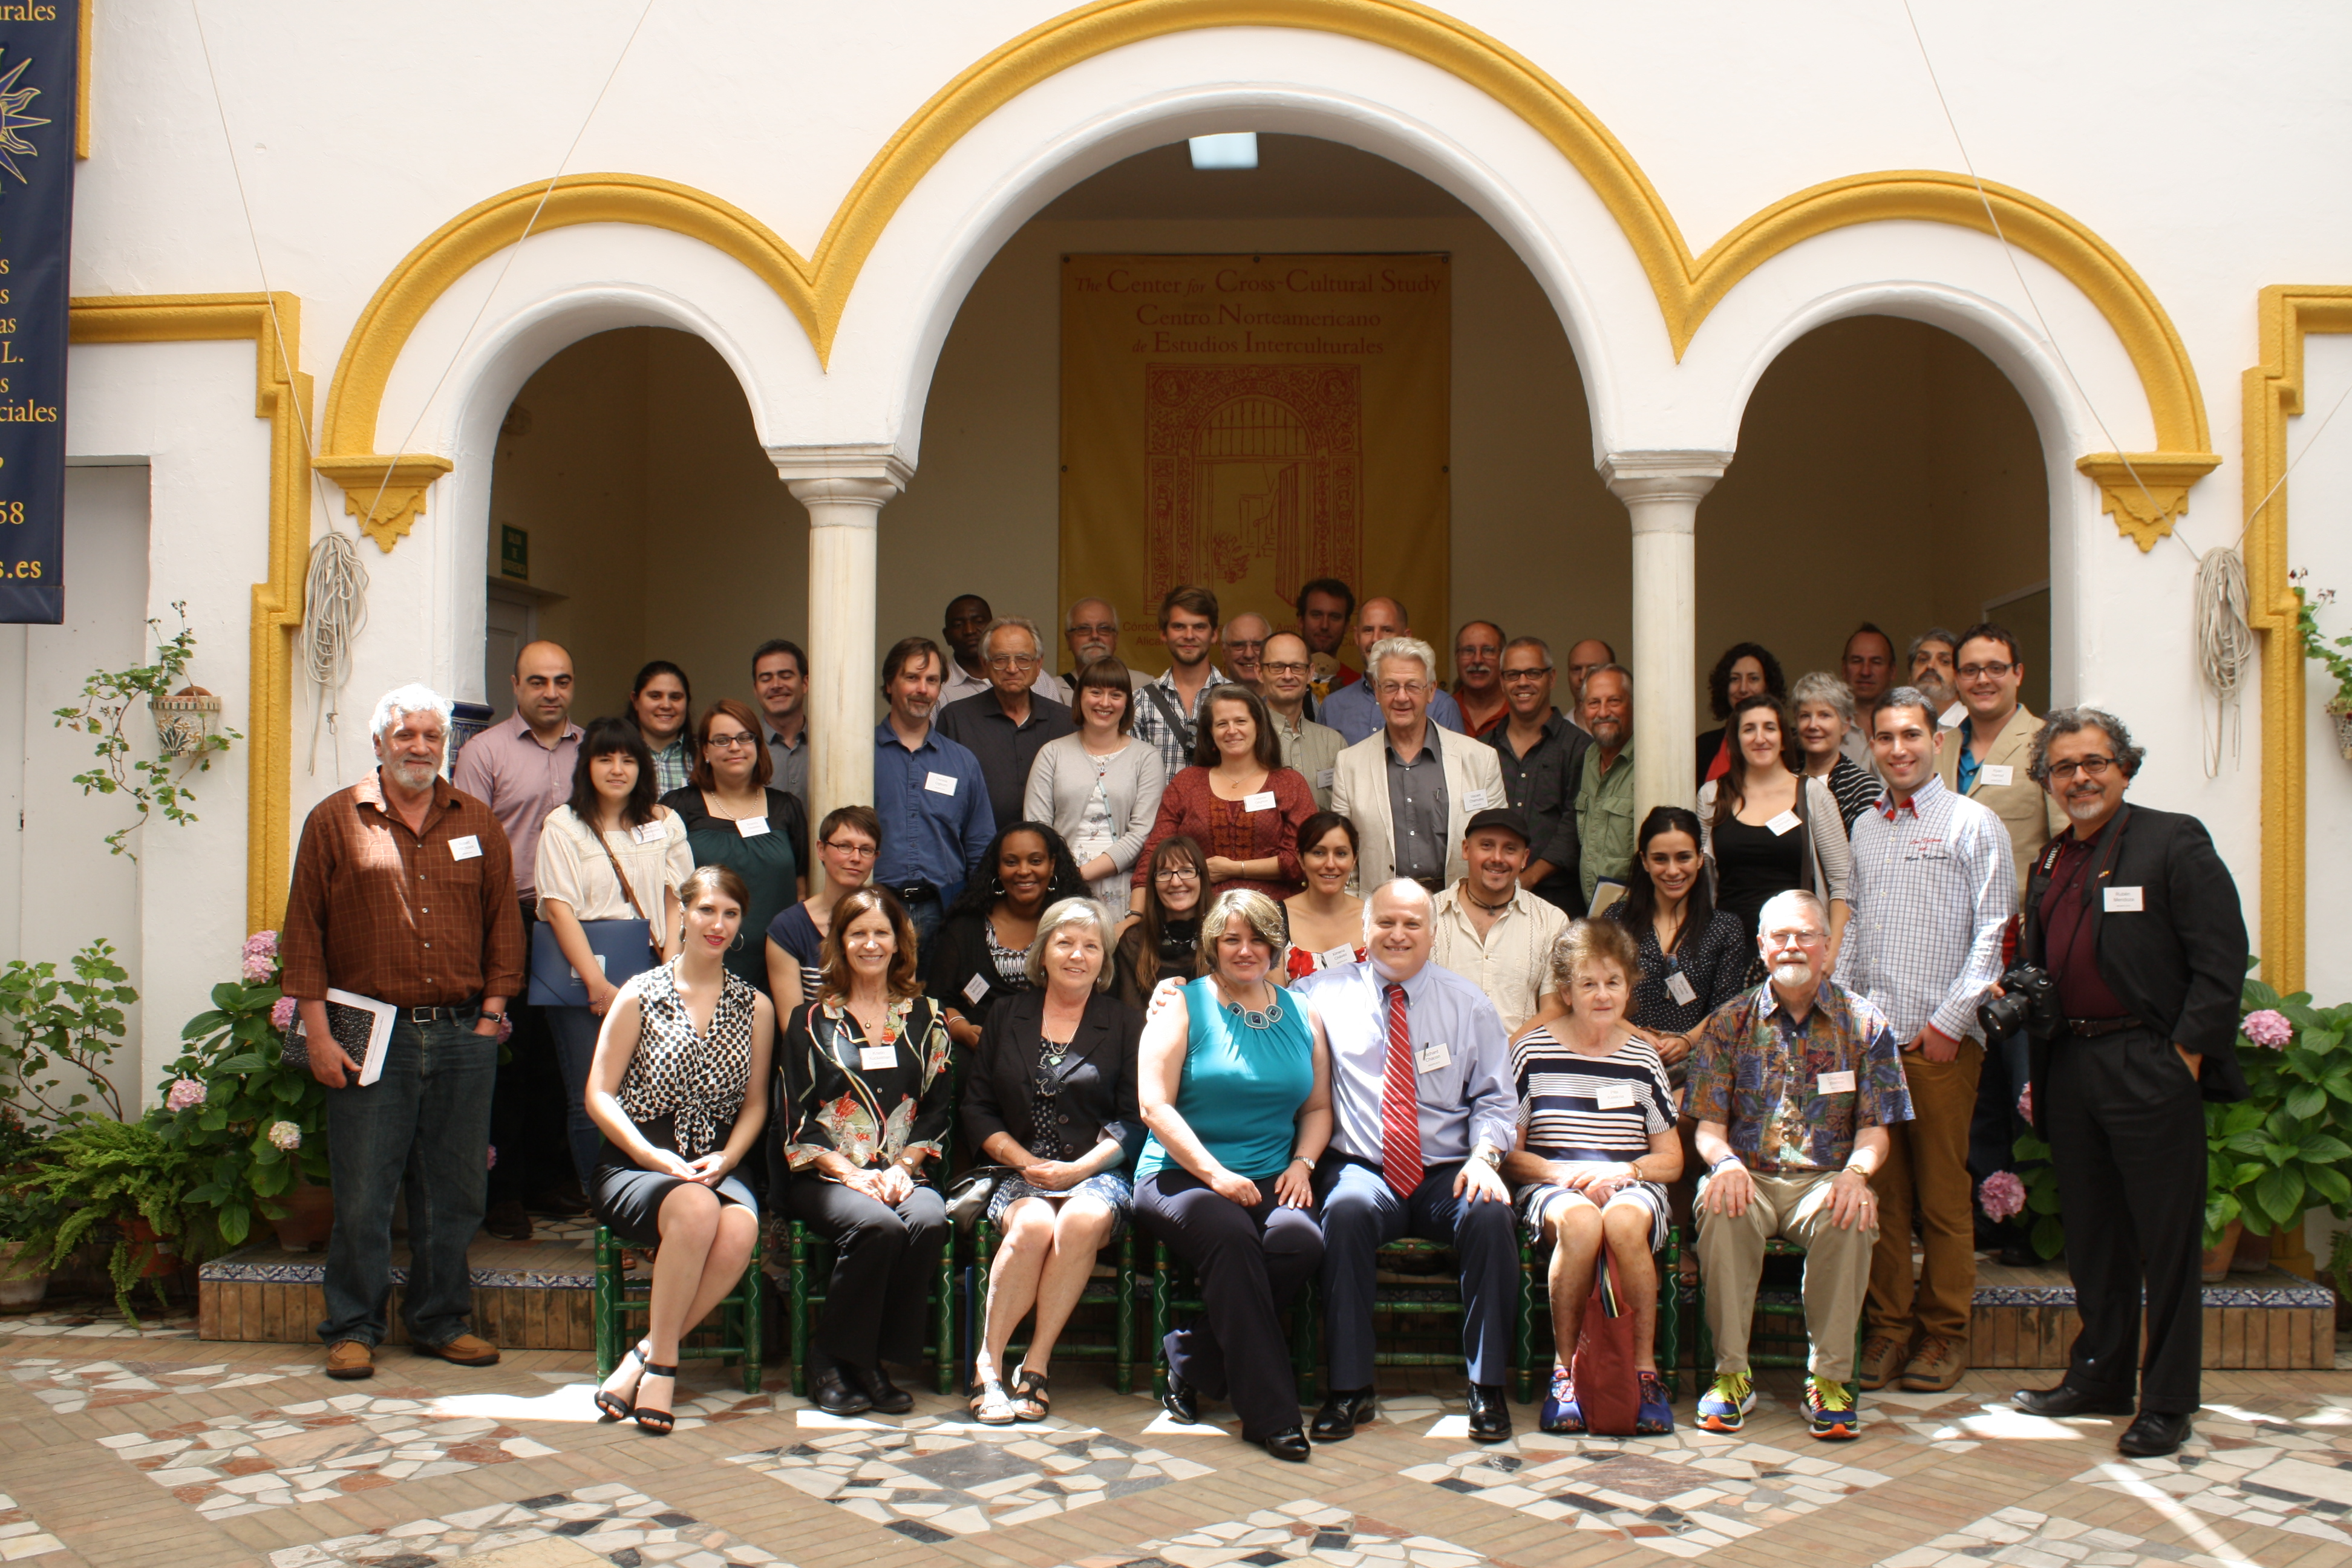
\includegraphics[width=\linewidth]{figures/WESIPS_Fig2.jpg}
		\centering
		\caption{Assistants to the WESIPS Conference, in the Andalusian patio of the Centre for Cross-Cultural Study, Seville. Courtesy of Dr. Richard Chacon.}
		\label{fig:WESIPS_Fig2}
	\end{figure}
In this conference a broad time and space spectrum was discussed. It promoted a stimulating dialogue amongst the conference participants, focused on how humans appropriate, manage and modify the environment, as well as how humans construct social relations of conflict and violence directed towards other human and non-human populations and landscapes. In this sense, the manifestations of violence are not confined to mankind but also include animals and the environment. The broad temporalities that were addressed during the conference made possible a debate on the various factors that regulate and promote the exercise of power and war.  It is clear that we need to encourage more events like this to exchange diverse points of view and to discuss the concepts of war, conflict and violence, all together. Fortunately, Richard and Yamilette have launched a new call to participate at the \href{https://www.academia.edu/14533728/WESIPS_2017_Conference}{2017 WESIPS Conference}, which will again be held in the wonderful city of Seville, Spain.  As in the first edition, this call is also opened to students interested in sharing their knowledge on these topics. We are sure that new proposals and discussions will help contribute to the field of warfare and environment, social inequality, and peace studies.





\label{WESIPS:lastpage}
\closingarticle
